\documentclass[main.tex]{subfiles}

\begin{document}
The goal of precision nuclear measurements is a test of the standard model.
If a parameter measured thus far to be zero is found to be non-zero, new physics would have been found. 
The usual window for low energy precision measurements is through beta decay.
The various precision measurements of beta decay are not the only method to look for new physics.

The most direct way to look for new physics is to look for the new particles that generate that physics.
One is to look for new particles with high energy experiments. 
The direct detection of new particles is very general and a powerful technique.
Precision measurements at high energies with colliders often done as well. 
 
Low energy precision measurements, on the other hand, are much more specialized.
Precision measurements are sensitive to only certain channels of new physics.
Care must be taken that the channel of physics is not covered by collider experiments already.
For nuclear physics searches, this is done by looking at beta decay, which provides a sensitive probe to several avenues of new physics.

\section{Beta Decay}
Beta decay is one of the processes by which unstable nuclei lose energy.
The general process is %shown in equation \ref{eq:betadecay}

\begin{equation}
	\label{eq:betadecay}
	^{A}_{Z}P \rightarrow ^{A}_{Z\pm 1}D + e^{\pm} + \nu_{e}
\end{equation}

with $^{A}_{Z}P$ being the parent nucleus, $^{A}_{Z \pm 1}D$ being the daughter nucleus, $e^{\pm}$ is the outgoing electron or positron, and $\nu$ is an outgoing neutrino.
The neutrino is an anti-electron neutrino in the case of beta$^{-}$ decay, and an electron neutrino in the case of beta$^{+}$ decay. 
There is also the process of electron capture, where a proton in the nucleus captures an inner electron and turns into a neutron.

The simplest type of nuclear beta decay is allowed beta decay.
There are two types of allowed beta decay, which differ in angular momentum $J$ and isospin $T$ selection rules.
The two types are called Fermi and Gamow-Teller beta decay. 
Neither of these transitions change parity.
The difference is that, in a Fermi transition, the change of the angular momentum $J$ and the change of the isospin $T$ is both zero.
For a Gamow-Teller transition, the change in the angular moment $J$ is $0$ or $\pm1$ and the change of the isospin $T$ is $0$ or $\pm 1$.
However, a Gamow-Teller transition cannot cause a transition between two states of $J = 0$. 
These are called super-allowed beta decays.
There are also mixed allowed transitions, where both matrix elements of Fermi decay and Gamow Teller decay contribute.
In order to see what physics beyond the standard model beta decay measurements are sensitive to, a closer look at beta decay is needed.

\subsection{Microscopic View of Beta Decay}
At a microscopic level, the process of beta decay involves one of the quarks inside the nucleon emitting a $W$ particle.
This quark changes flavor, and the nucleon changes as well. 
The microscopic view of beta decay (for the beta$^{-}$ case) is shown in figure \ref{fig:betadecaymicro}.

\begin{figure}[!htb]
	\centerline{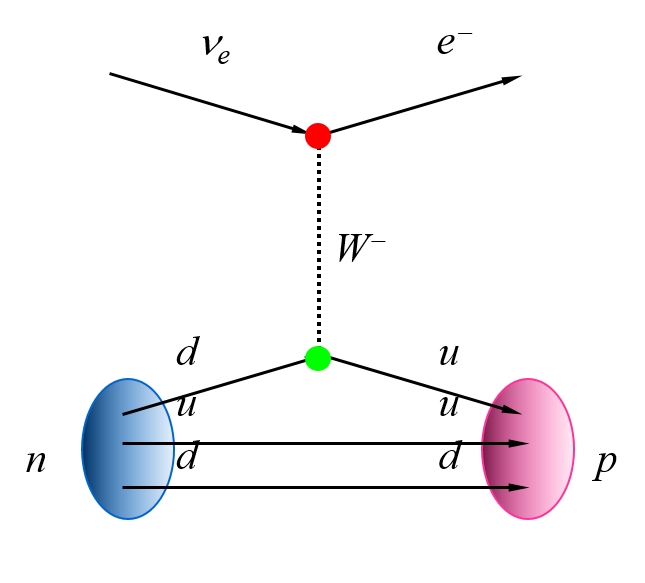
\includegraphics[width=0.5\textwidth]{fig_betadecayzoomedin.png}}
	\caption{What beta$^{-}$ decay looks like microscopically}
	\label{fig:betadecaymicro}
\end{figure}

A down quark in a neutron goest to an up quark.
This process emits a $W^{-}$ boson that decays into an electron and an anti-electron neutrino.
This means that any beta decay measurements are probing the weak sector. 
These measurements are complimentary to high energy measurements of weak interactions.
For this work, a nucleon level treatment of beta decay will suffice.  

\subsection{Matrix elements of Beta Decay}
In order to calculate the beta decay rate, Fermi's golden rule is needed.
This is %shown as in equation \ref{eq:fgr}.

\begin{equation}
	\lambda = \frac{2\pi}{\hbar}\|M\|^{2}\rho(E)
	\label{eq:fgr}
\end{equation}

The density of states, $\rho(E)$, will be discusses further in the thesis. 

This matrix element $M$, to first order, is \cite{Gon19} %shown in equation \ref{eq:matrixelement} \cite{Gon19}

\begin{equation}
	|M|^{2} = \xi [1 + a \frac{\vec{p_{e}} \cdot \vec{p_{\nu}}} {E_{e} E_{\nu}}  +  b \frac{m_{e}}{E_{e}} + \frac{\vec{<J>}}{J} \cdot (A \frac{ \vec{p_{e}} }{E_{e}} + B \frac{\vec{p_{\nu}}}{E_{\nu}} + D \frac{\vec{p_{e}} \times \vec{p_{\nu}}}{E_{e} E_{\nu}})]
	\label{eq:matrixelement}
\end{equation}

$\xi$ is written out to linear order is %in equation \ref{eq:xiwrittenout}. 
 
\begin{equation}
	\xi = \frac{1}{2} |M_{F}|^{2} |C_{V} + C'_{V}|^{2} (1 + |\rho|^{2})
	\label{eq:xiwrittenout}
\end{equation}

For equation \ref{eq:xiwrittenout}, $M_{F}$ is the Fermi matrix element, $C_{V}$ and $C_{V}$ are vector coupling constants, and $|\rho|$ is the ratio of the Gamow-Teller matrix element to the Fermi matrix element.
\cite{Gon19}

Going back to equation \ref{eq:decayrate}, $<\vec{J}>$ is the average total angular momentum. 
The constants $a$, $b$, $A$, $B$, and $D$ can be written in terms of the coupling constants as well.
$a$ depends on the ratio of the Fermi and Gamow-Teller matrix elements $\rho$.
This form of the observables informs the experimental design. 

\section{Types of Precision Measurements in Beta Decay}
Given the form of equation \ref{eq:decayrate}, to get at different terms, different types of experiments are needed.
A polarized nucleus is need to extract $a$. 
The nuclear spin points in one direction. 
Then, by angular momentum conservation, $\vec{p_{e}} \cdot \vec{p_{\nu}}$ can be found.
Other correlations between energy and momenta have sensitivity to other terms in equation \ref{eq:decayrate}.
Equation \ref{eq:decayrate} is not complete, and many other terms exist. 

For an unpolarized beam where only the energy of the electron is measured, the momenta are averaged over and all terms disappear expect for $b$.
There is also the phase space factor.
There are two general kinds of unpolarized beta decay measurements.
The first is where the differential energy spectrum is measured.
There is a measurement of $b$ over the entire range of values, and the $\frac{1}{W}$ dependence of the matrix element is probed.
To do this measurement, the beta decay in question must be available enough in order to get enough statistics for a good spectrum.
Other requirements for a spectrum shape measurement are described in the next chapter.

If the nucleus is rare, another way to get at the physics in equation \ref{eq:decayrate} is to measure an $ft$ value.
The $f$ is the integral of the decay rate.
The $t$ is the half-life of the nucleus times the branching ratio.
These are both measured and multiplied together to get a quantity that is proportional to the matrix element.
This can be done even if the nucleus in question is difficult to produce.
For each measurement, $b$ is measured, but modulated by an average value of the energy dependence.
Multiple measurements are needed to get good constraints on $b$.

In both of these techniques, electromagnetic and hardonic corrections are needed.
To measure the $ft$ values, the integral of these corrections are important.
For the shape measurements, the energy dependence of the corrections are important.
The systematic uncertainties for both of the techniques are different.
These depend on the exact details of the experiment.

The term $b$ is known and the Fierz interference term.
A measurement of this term is the ultimate goal of the experiment described in this thesis.
A more detailed discussion of the term is needed.

\subsection{Fierz Term}
The Fierz term, $b$, in equation \ref{eq:decayrate}, can be rewritten in terms of effective couplings.
This is %shown in equation \ref{eq:bwrittenout}

\begin{equation}
	b =  \pm \sqrt{1 - \alpha^{2}{Z^{2}}}\frac{1}{1 + \rho}Re(\frac{C_{S} + C_{S}'}{C_{V} + C_{V}'} + |\rho|^{2}\frac{C_{T} + C_{T}'}{C_{A} + C_{A}'})
	\label{eq:bwrittenout}
\end{equation}

where $\rho$ is the ratio of the Gamow-Teller matrix element to Fermi matrix element, $\alpha$ is the QED fine structure constant \cite{Gon19}
The subscripts of $C$ indicate which object the coupling corresponds to. 
Here, $A$ means axial vector, $V$ stands for polar vector, $S$ stands for scalar, and $T$ stands for tensor. 
The $C$ coefficients correspond to parity conserving interactions, and the $C'$ coefficients correspond to parity non-conserving coefficients \cite{Lee56}
This means, that in a pure Fermi decay, the Fierz term is sensitive to any non-standard scalar term, while in a pure Gamow-Teller decay, the Fierz term is sensitive to any non-standard Tensor terms. 

The Fermi decays have been measured using super-allowed beta decays.
For most of these measurements, however, decay of interest happens very rarely.
The $ft$ value was measured.
$ft$ values give the value of the Fierz term averaged over the beta decay energy spectrum.
Several measurements of different decays are needed to get a good constraint.
The other part of the Fierz term is the tensor coupling. 
In order to get a good measurement of  tensor couplings, an allowed Gamow-Teller decay must be used. 
The nucleus for this measurement was $^{20}$F.
This measurement was done carefully to compete with high energy probes.

\subsection{High Energy Probes of the Fierz Term}

There have been probes sensitive to the Fierz term done with high energy techniques \cite{Gon19}.
The precision of these measurements is important to keep in mind, as this is the precision goal of the beta decay measurement.
Several high-energy channels are used, and the coupling chagres are directly measured.
To compare the results of the channels to a precision beta decay measurement, the Fierz terms needs to be rewritten.
In the case of a Gamow-Teller transition, the Fierz term in equation \ref{eq:bwrittenout} can be re-written to %equation \ref{eq:bgt}

\begin{equation}
	b_{gt} = \pm 2 \sqrt{1 - \alpha^{2} Z^{2}} Re(\frac{C_{T} + C_{T}'}{C_{A} + C_{A}'})
	\label{eq:bgt}
\end{equation}

In terms of the quark level coupling constants, this can be rewritten as \cite{Gon19} %shown in equation \ref{eq:bgtquarklevel} \cite{Gon19}

\begin{equation}
	b_{gt} = \pm 2 \sqrt{1 - \alpha^{2} Z^{2}} Re(\frac{8 g_{t} \epsilon_{t}}{2 g_{A}})
	\label{eq:bgtquarklevel}
\end{equation}

with $g_{t}$ being the tensor charge, $\epsilon_{t}$ the tensor coupling and $g_{A}$ the axial vector charge.
This is assuming the only physics beyond the standard model is in $\epsilon_{t}$.
The value of $g_{t}$ is $0.987(55)$ and $g_{A} = 1.278 (33)$ \cite{Gon19}.
This means, for $^{20}$F, the sensitvity to $b_{gt}$ in terms of $\epsilon_{t}$ is given by %equation \ref{eq:bgtpropor}

\begin{equation}
	b_{gt} = \pm 6.2 * Re(\epsilon_{t})
	\label{eq:bgtpropor}
\end{equation}
This can be used to describe the ultimate sensitivity needed.

For the high energy probes, the Large Hardon Collider collides two protons and looks at the output. 
The experimental signature for the LHC is missing transverse energy.
The energy of the output particles is compared to that of the standard model background, and the difference recorded.
To probe the same physics as beta decay, one or more of the outgoing particles are electrons or positrons.
For events with one electron and other particles, the constraint on $\epsilon_{t}$ is $|\epsilon_{t}| < 1.3 \times 10^{-3}$.
Looking at neutral currents, where the output particles include an electron and a positron, gives stronger constraints.
There, the constraint is $|\epsilon_{t}| < 0.6 \times 10^{-3}$.
To be competitive with the stronger constraint from high energy experiments, the Fierz term $b_{gt}$ should be measured to better than $3.7 \times 10^{-3}$. 


In order to achieve such a measurement, the technique used was a shape measurement technique.
The next chapter will describe why this method works with a measurement of $^{20}$F.

\end{document}
